% Provenance (never printed): lycee terminale S SVT "Les climats de la Terre"
% and the 2019 enseignement scientifique ("Le climat de la Terre": forcing,
% feedbacks, the IPCC assessments, scenarios), union; physical science only,
% as the user ruled (2026-10-22). See sources/outline_sources.md. Pilot
% chapter, 2026-10-22. Every figure about the climate system is an IPCC AR6
% WG1 statement (ledger ipcc:*) or computed from a dataset in
% figdata/grade-12/climate_records.py.
\chapter{A mudança do clima: observações, causas e projeções}\label{ch:g12:climate-change}

No alto da encosta norte do Mauna Loa, um vulcão no meio do oceano Pacífico,
um conjunto de prédios brancos se ergue sobre a lava nua, a \qty{3397}{m}
acima do mar. Lá em cima, acima da camada de ar poluída pela ilha abaixo e a
milhares de quilômetros de qualquer grande cidade, o ar é quase tão limpo e
bem misturado quanto a atmosfera do planeta inteiro. Desde março de 1958, o
seu gás carbônico é medido quase sem interrupção. O registro começou como o
projeto de um químico; ele se tornou a curva mais famosa das ciências da
Terra. Este capítulo lê essa curva e os outros registros do clima, explica
como uma mudança no ar muda o \omterm{def:g10:earth-energy-budget:energy-budget}{balanço de energia} do planeta, como os
cientistas decidem o que causou o aquecimento que eles observam, e o que
eles projetam para as próximas décadas.
% ledger: noaa:mlo-site, noaa:keeling-1958

\begin{omfigure}
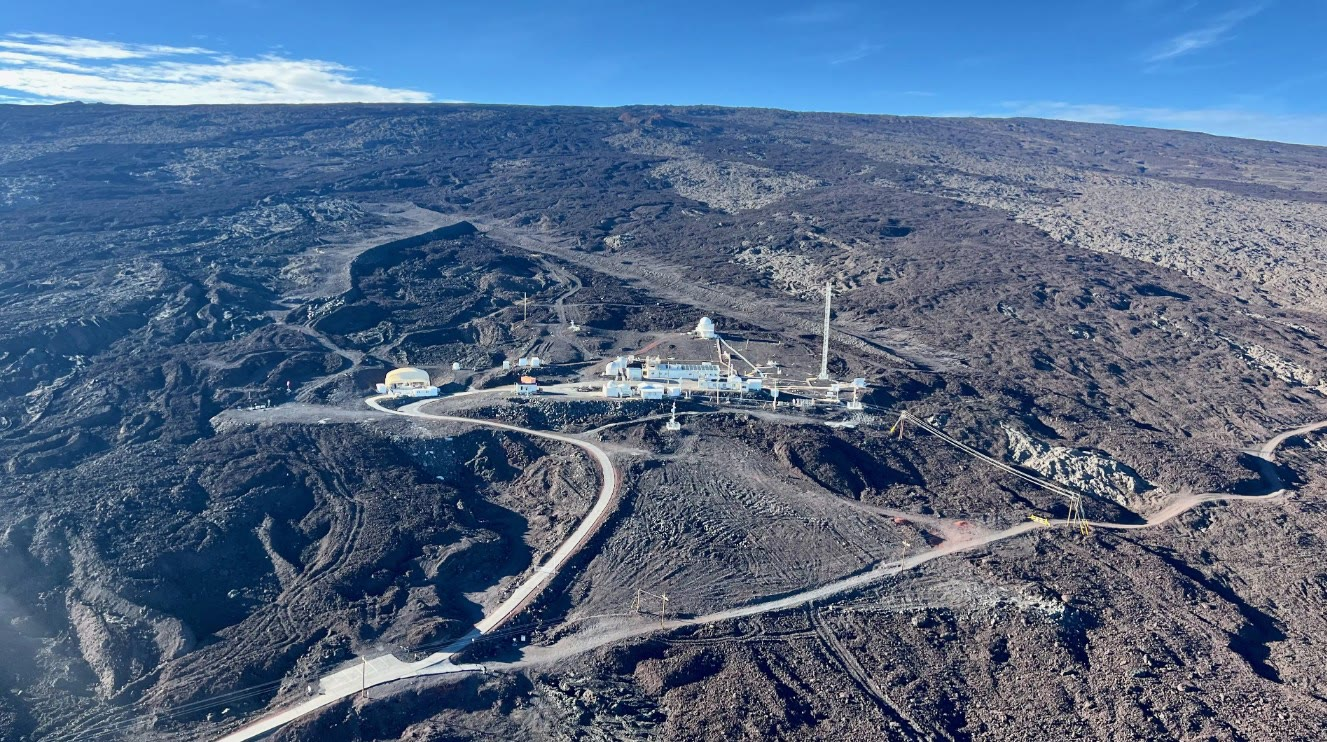
\includegraphics[width=0.78\linewidth]{images/book2/g12-noaa-mauna-loa-observatory.jpg}

{\small O Observatório de Mauna Loa, no Havaí, sobre antigos derrames de lava
no alto do flanco norte do vulcão. Fotografia: Brian Vasel, NOAA (domínio
público).}
\end{omfigure}

\begin{recall}
A Terra recebe energia do Sol como luz e perde a mesma quantidade, em média,
para o espaço como radiação infravermelha; a fração da luz do Sol refletida
é o \omterm{def:g10:earth-energy-budget:albedo}{albedo} (\cref{ch:g10:earth-energy-budget}). Os gases de efeito estufa
--- vapor de água, gás carbônico, metano --- absorvem parte do infravermelho
que a superfície emite e devolvem parte dele para baixo; esse efeito estufa
mantém a superfície muito mais quente do que ela seria sem ele (os livros de
química, e o Livro 1, 9º ano). Os \omterm{def:g12:past-climates:ice-core}{testemunhos de gelo} guardam bolhas de ar
antigo e registram os \omterm{def:g12:past-climates:glacial-cycle}{ciclos glaciais} dos últimos 800\,000 anos
(\cref{ch:g12:past-climates}).
\end{recall}

\section{Os registros}

\begin{omfigure}
\begin{tikzpicture}
\begin{axis}[omrecord, width=0.92\linewidth, height=6.2cm, xmin=1957, xmax=2028,
  ymin=305, ymax=440, xlabel={ano}, ylabel={gás carbônico (ppm)},
  xtick={1960,1970,...,2020}, /pgf/number format/1000 sep={}]
\addplot[omDef!85!black, line width=0.5pt] table[x=decimal_year, y=co2_ppm] {figdata/out/grade-12-climate_records-co2.dat};
\addplot[only marks, mark=*, mark size=0.9pt, omThm!85!black] table[x=year, y=co2_ppm] {figdata/out/grade-12-climate_records-co2annual.dat};
\end{axis}
\end{tikzpicture}

{\small O teor de gás carbônico do ar em Mauna Loa: médias mensais (linha) e
médias anuais (pontos), em partes por milhão (ppm) de ar seco. Dados: NOAA
Global Monitoring Laboratory e Scripps Institution of Oceanography.}
\end{omfigure}

\begin{proposition}[O registro do gás carbônico]\label{prop:g12:climate-change:co2}
% ledger: data:co2-mlo (all numbers computed in figdata/grade-12/climate_records.py)
Em Mauna Loa, a concentração média anual de gás carbônico subiu de
\qty{316.0}{ppm} em 1959 para \qty{427.4}{ppm} em 2025, e a subida está se
acelerando: a concentração cresceu cerca de \qty{0.9}{ppm} por ano na década
de 1960 e cerca de \qty{2.6}{ppm} por ano entre 2015 e 2025. Todo ano, a
concentração também oscila cerca de \qty{7}{ppm}: ela é máxima em maio e
mínima em setembro.
\end{proposition}

\begin{remark}[Por que a curva tem dentes]\label{rem:g12:climate-change:teeth}
A oscilação anual é a respiração da vegetação do Hemisfério Norte, onde está
a maior parte das plantas terrestres. Na primavera e no verão, as plantas
absorvem pela fotossíntese mais gás carbônico do que elas e o solo liberam;
no outono e no inverno, a decomposição e a respiração vencem. A subida de um
ano para o outro é outra história: é o carbono dos combustíveis fósseis e
das florestas derrubadas se acumulando no ar.
\end{remark}

\begin{proposition}[Mais alto do que em pelo menos dois milhões de anos]\label{prop:g12:climate-change:icecore}
% ledger: data:co2-bereiter (173.7 and 298.6 ppm computed), ipcc:co2-2myr (high confidence)
Ao longo dos últimos 800\,000 anos, as bolhas de ar do gelo antártico
registram concentrações de gás carbônico entre cerca de \qty{174}{ppm}, nos
\omterm{def:g12:past-climates:glacial-cycle}{períodos glaciais} mais frios, e \qty{299}{ppm}, nos \omterm{def:g12:past-climates:glacial-cycle}{interglaciais} mais
quentes. O valor de hoje fica mais de \qty{100}{ppm} acima do mais alto
deles. As avaliações afirmam que a concentração em 2019 era mais alta do que
em qualquer momento de pelo menos os últimos dois milhões de anos
(\emph{alta confiança}).
\end{proposition}

\begin{omfigure}
\begin{tikzpicture}
\begin{axis}[omrecord, omage, width=0.92\linewidth, height=5.2cm, xmin=0, xmax=810,
  ymin=150, ymax=490, xlabel={milhares de anos antes de 1950},
  ylabel={gás carbônico (ppm)}, xtick={0,100,...,800}]
\addplot[omDef!85!black, line width=0.6pt] table[x=age_kyr, y=co2_ppm] {figdata/out/grade-12-climate_records-icecore.dat};
\draw[omThm, densely dashed, line width=0.8pt] (axis cs:810,427.35) -- (axis cs:0,427.35);
\node[font=\footnotesize, text=omThm!85!black, anchor=south west] at (axis cs:780,433) {média anual em Mauna Loa em 2025};
\end{axis}
\end{tikzpicture}

{\small O gás carbônico do gelo antártico ao longo de 800\,000 anos: os
\omterm{def:g12:past-climates:glacial-cycle}{ciclos glaciais} o fazem variar entre cerca de 180 e \qty{300}{ppm}. O pico
fino na extremidade direita é o gelo mais jovem, que registra o início da
subida atual, até o ano de 2001. Dados: Bereiter e colaboradores (2015),
NOAA Paleoclimatology.}
% the youngest sample of the composite: age -51 yr BP (2001), 368.02 ppm (data/derived/co2-icecore.csv)
\end{omfigure}

\begin{omfigure}
\begin{tikzpicture}
\begin{axis}[omrecord, width=0.92\linewidth, height=5.6cm, xmin=1878, xmax=2027,
  ymin=-0.6, ymax=1.45, xlabel={ano},
  ylabel={anomalia de temperatura (\unit{\degreeCelsius})},
  xtick={1880,1900,...,2020}, /pgf/number format/1000 sep={},
  legend style={at={(0.03,0.96)}, anchor=north west, font=\footnotesize, draw=black!30}]
\addplot[omDef!70, line width=0.5pt, mark=*, mark size=0.6pt] table[x=year, y=anomaly] {figdata/out/grade-12-climate_records-temp.dat};
\addlegendentry{média anual}
\addplot[omThm!85!black, line width=1.3pt, unbounded coords=jump] table[x=year, y=mean11] {figdata/out/grade-12-climate_records-temp.dat};
\addlegendentry{média de 11 anos}
\end{axis}
\end{tikzpicture}

{\small A temperatura média global da superfície, como diferença em relação
à sua média de 1951--1980. Dados: NASA GISS Surface Temperature Analysis
(GISTEMP v4).}
\end{omfigure}

\begin{proposition}[O aquecimento global observado]\label{prop:g12:climate-change:warming}
% ledger: ipcc:gsat-2011-2020, ipcc:decades
Cada uma das últimas quatro décadas foi mais quente que qualquer década
anterior desde 1850. A temperatura global da superfície de 2011--2020 foi
\qty{1.09}{\degreeCelsius} mais alta que a de 1850--1900 (muito
provavelmente entre 0.95 e \qty{1.20}{\degreeCelsius}), com mais aquecimento
sobre os continentes (\qty{1.59}{\degreeCelsius}) que sobre o oceano
(\qty{0.88}{\degreeCelsius}).
\end{proposition}

\begin{proposition}[O nível do mar sobe cada vez mais depressa]\label{prop:g12:climate-change:sea}
% ledger: ipcc:sea-level-obs, data:gmsl-lsa (3.2 mm/yr trend computed)
O nível médio global do mar subiu cerca de \qty{0.20}{m} entre 1901 e 2018.
A taxa foi de cerca de \qty{1.3}{mm} por ano de 1901 a 1971,
\qty{1.9}{mm} por ano de 1971 a 2006 e \qty{3.7}{mm} por ano de 2006 a 2018
(\emph{alta confiança}). Os satélites, que medem a altura da superfície do
mar desde 1993, encontram uma média de \qty{3.2}{mm} por ano em 1993--2025.
O mar sobe porque o oceano, ao se aquecer, se dilata, e porque as geleiras e
os mantos de gelo perdem gelo para ele.
\end{proposition}

\begin{omfigure}
\begin{tikzpicture}
\begin{axis}[omrecord, width=0.86\linewidth, height=5cm, xmin=1992, xmax=2026,
  ymin=-35, ymax=95, xlabel={ano}, ylabel={nível do mar (mm)},
  /pgf/number format/1000 sep={}, xtick={1995,2000,...,2025}]
\addplot[omDef!85!black, line width=0.5pt] table[x=decimal_year, y=gmsl_mm] {figdata/out/grade-12-climate_records-sea.dat};
\end{axis}
\end{tikzpicture}

{\small O nível médio global do mar medido do espaço, mais ou menos a cada
dez dias (sinal sazonal removido), em relação a um zero arbitrário. Dados de
altimetria fornecidos pelo NOAA Laboratory for Satellite Altimetry.}
\end{omfigure}

\begin{dated}{2025}
% ledger: data:co2-mlo, data:gistemp (values read from the datasets as fetched 2026-10-22)
A concentração média anual de gás carbônico em Mauna Loa em 2025 foi de
\qty{427.35}{ppm}. No registro de temperatura da NASA, o ano mais quente até
agora foi 2024, a \qty{1.28}{\degreeCelsius} acima da média de 1951--1980.
\end{dated}

\section{O forçamento radiativo}

\begin{definition}[Forçamento radiativo]\label{def:g12:climate-change:forcing}
O \emph{forçamento radiativo}\index{forcamento radiativo@forçamento radiativo} de uma mudança no
sistema climático --- mais gás de efeito estufa, mais partículas de
aerossóis, um Sol mais brilhante --- é a variação que ela causa no fluxo
líquido de energia que entra no sistema climático no topo da atmosfera,
antes que a temperatura da superfície tenha tido tempo de responder. Ele é
medido em watts por metro quadrado (\unit{W/m^2}) da superfície da Terra.
Um forçamento positivo faz o planeta ganhar energia e se aquecer; um
forçamento negativo o faz perder energia e se resfriar.
\end{definition}

\begin{remark}[Forçamento efetivo]\label{rem:g12:climate-change:effective}
As avaliações usam o \omterm{def:g12:climate-change:forcing}{forçamento radiativo} \emph{efetivo}, que conta também
os ajustes rápidos da atmosfera (das suas nuvens, por exemplo) que
acontecem antes que a superfície se aqueça. Todos os \omterm{def:g12:climate-change:forcing}{forçamentos} deste
capítulo são \omterm{def:g12:climate-change:forcing}{forçamentos} efetivos.
\end{remark}

\begin{proposition}[O forçamento desde 1750]\label{prop:g12:climate-change:forcing}
% ledger: ipcc:erf-total, ipcc:erf-agents
As atividades humanas produziram um \omterm{def:g12:climate-change:forcing}{forçamento radiativo} total de
\qty{2.72}{W/m^2} em 2019 em relação a 1750 (muito provavelmente entre 1.96
e \qty{3.48}{W/m^2}). Os gases de efeito estufa contribuem com um \omterm{def:g12:climate-change:forcing}{forçamento}
positivo, liderado pelo gás carbônico (\qty{2.16}{W/m^2}); as partículas de
aerossóis, que refletem a luz do Sol e clareiam as nuvens, contribuem com um
\omterm{def:g12:climate-change:forcing}{forçamento} negativo (cerca de \qty{-1.06}{W/m^2} ao todo). A variação do
brilho do Sol no mesmo período contribui com apenas \qty{0.01}{W/m^2}.
\end{proposition}

\begin{omfigure}
% ledger: ipcc:erf-agents, ipcc:erf-total (central values and 5-95 % ranges of AR6 Table 7.8)
\begin{tikzpicture}
\begin{axis}[xbar, width=0.8\linewidth, height=7.2cm, xmin=-1.8, xmax=3.7,
  ytick={1,...,10}, yticklabels={total (humano), solar, uso da terra,
  aerossóis--nuvens, aerossóis--radiação, ozônio, gases halogenados, óxido nitroso,
  metano, gás carbônico}, y tick label style={font=\small},
  tick label style={font=\small}, xlabel={forçamento radiativo efetivo, 1750--2019 (\unit{W/m^2})},
  label style={font=\small}, bar width=6pt, bar shift=0pt, axis x line=bottom, axis y line=left,
  axis line style={-}, enlarge y limits=0.07, xmajorgrids,
  grid style={gray!22, line width=0.3pt}, extra x ticks={0},
  extra x tick style={grid style={black!60, line width=0.5pt}}]
\addplot[fill=omThm!55, draw=omThm!80!black, error bars/.cd, x dir=both, x explicit,
  error bar style={black!70}] coordinates {
  (2.16,10) += (0.25,0) -= (0.26,0)
  (0.54,9) += (0.11,0) -= (0.11,0)
  (0.21,8) += (0.03,0) -= (0.03,0)
  (0.41,7) += (0.08,0) -= (0.08,0)
  (0.47,6) += (0.24,0) -= (0.23,0)
  (2.72,1) += (0.76,0) -= (0.76,0)
  (0.01,2) += (0.07,0) -= (0.07,0)};
\addplot[fill=omDef!55, draw=omDef!80!black, error bars/.cd, x dir=both, x explicit,
  error bar style={black!70}] coordinates {
  (-0.22,5) += (0.26,0) -= (0.25,0)
  (-0.84,4) += (0.59,0) -= (0.61,0)
  (-0.20,3) += (0.10,0) -= (0.10,0)};
\end{axis}
\end{tikzpicture}

{\small Os principais \omterm{def:g12:climate-change:forcing}{forçamentos radiativos} efetivos de 1750 a 2019, com as
suas faixas muito prováveis (barras de erro). Valores: Sexto Relatório de
Avaliação do IPCC, Grupo de Trabalho~I, Tabela 7.8.}
\end{omfigure}

\begin{proposition}[O gás carbônico: cada duplicação acrescenta o mesmo forçamento]\label{prop:g12:climate-change:log}
% ledger: ipcc:erf-2xco2, ipcc:log-co2
Numa boa aproximação, o \omterm{def:g12:climate-change:forcing}{forçamento} do gás carbônico cresce com o
\emph{logaritmo} da sua concentração: cada duplicação acrescenta o mesmo
\omterm{def:g12:climate-change:forcing}{forçamento}, $F_{2\times} = \qty{3.93}{W/m^2}$ para uma duplicação a partir da
concentração de 1750, $C_0 = \qty{278}{ppm}$. O \omterm{def:g12:climate-change:forcing}{forçamento} de uma
concentração $C$ é então
\[
  F = F_{2\times}\,\frac{\ln (C/C_0)}{\ln 2}.
\]
\end{proposition}

\begin{example}[Verificar a lei com a avaliação]\label{ex:g12:climate-change:check}
% ledger: ipcc:erf-2xco2, ipcc:erf-agents
Em 2019, a concentração era de \qty{410}{ppm}. A lei dá
$F = 3.93 \times \ln(410/278)/\ln 2 = 3.93 \times 0.561 \approx
\qty{2.20}{W/m^2}$, a menos de 2\,\% dos \qty{2.16}{W/m^2} que a
avaliação dá para o gás carbônico em 1750--2019.
\end{example}

\begin{proposition}[Para onde vai a energia extra]\label{prop:g12:climate-change:heating}
% ledger: ipcc:heating
Como o \omterm{def:g12:climate-change:forcing}{forçamento} é positivo, o sistema climático ganha energia: cerca de
\qty{0.79}{W/m^2} em média em 2006--2018, contra \qty{0.50}{W/m^2} em
1971--2006 (\emph{alta confiança}). O oceano recebeu 91\,\% dessa energia;
os continentes 5\,\%, o gelo que derrete 3\,\% e a atmosfera apenas 1\,\%.
\end{proposition}

\section{Retroalimentações e sensibilidade climática}

Quando a superfície se aquece, ela irradia mais energia para o espaço, o que
tende a trazer o planeta de volta ao equilíbrio. Mas o aquecimento também
muda outras coisas --- o vapor de água do ar, a neve e o gelo no solo, as
nuvens ---, e essas mudanças alteram por sua vez o \omterm{def:g10:earth-energy-budget:energy-budget}{balanço de energia}.

\begin{definition}[Retroalimentação climática]\label{def:g12:climate-change:feedback}
Uma \emph{retroalimentação climática}\index{retroalimentacao climatica@retroalimentação climática} é uma mudança no
sistema climático, causada por uma variação de temperatura, que altera o
\omterm{def:g10:earth-energy-budget:energy-budget}{balanço de energia} e, portanto, a própria variação de temperatura. Uma
\emph{retroalimentação positiva} amplifica a mudança inicial; uma
\emph{retroalimentação negativa} a amortece.
\end{definition}

\begin{example}[Três retroalimentações]\label{ex:g12:climate-change:three}
\begin{itemize}
  \item \textbf{Vapor de água (positiva).} Um ar mais quente contém mais
        vapor de água, um gás de efeito estufa, o que reforça o aquecimento.
  \item \textbf{Neve e gelo (positiva).} A neve e o gelo refletem a luz do
        Sol; quando eles derretem, o solo e o mar mais escuros embaixo
        absorvem mais dela, e o aquecimento aumenta.
  \item \textbf{Radiação para o espaço (negativa).} Uma superfície e uma
        atmosfera mais quentes irradiam mais infravermelho para o espaço.
        Essa resposta básica sempre vence no fim: é por isso que o clima se
        estabiliza num novo equilíbrio, mais quente, em vez de se aquecer
        sem limite.
\end{itemize}
\end{example}

\begin{omfigure}
\begin{tikzpicture}[font=\small, >={Stealth[length=2.4mm]},
  box/.style={draw=black!60, rounded corners=2pt, fill=white, align=center,
  inner sep=3pt, text width=3cm}]
  \node[box, fill=omThm!12] (w) at (0,0) {a superfície se aquece};
  \node[box] (v) at (3.6,1.3) {mais vapor de água no ar};
  \node[box] (g) at (3.6,-1.3) {efeito estufa\\mais forte};
  \draw[->, omThm!85!black, thick] (w) to[bend left=18] (v);
  \draw[->, omThm!85!black, thick] (v) -- (g);
  \draw[->, omThm!85!black, thick] (g) to[bend left=18] (w);
  \node[font=\footnotesize, text=omThm!85!black] at (2.0,0) {$+$};
  \node[box] (s) at (-3.6,1.3) {a neve e o gelo derretem};
  \node[box] (a) at (-3.6,-1.3) {albedo mais baixo: mais luz do Sol absorvida};
  \draw[->, omThm!85!black, thick] (w) to[bend right=18] (s);
  \draw[->, omThm!85!black, thick] (s) -- (a);
  \draw[->, omThm!85!black, thick] (a) to[bend right=18] (w);
  \node[font=\footnotesize, text=omThm!85!black] at (-2.0,0) {$+$};
  \node[box] (r) at (0,-2.9) {mais infravermelho irradiado para o espaço};
  \draw[->, omDef!85!black, thick] ([xshift=-0.35cm]w.south) -- ([xshift=-0.35cm]r.north);
  \draw[->, omDef!85!black, thick] ([xshift=0.35cm]r.north) -- ([xshift=0.35cm]w.south);
  \node[font=\footnotesize, text=omDef!85!black] at (0.62,-1.45) {$-$};
\end{tikzpicture}

{\small Duas \omterm{def:g12:climate-change:feedback}{retroalimentações} positivas (laços vermelhos) amplificam um
aquecimento; o infravermelho extra irradiado por um planeta mais quente (em
azul) é uma \omterm{def:g12:climate-change:feedback}{retroalimentação} negativa que o limita.}
\end{omfigure}

\begin{proposition}[O aquecimento no equilíbrio]\label{prop:g12:climate-change:equilibrium}
% ledger: ipcc:feedbacks
Uma vez que o clima tenha atingido um novo equilíbrio, o aquecimento
$\Delta T$ causado por um \omterm{def:g12:climate-change:forcing}{forçamento} constante $F$ é
\[
  \Delta T = \frac{F}{\lambda},
\]
em que $\lambda$, o \emph{parâmetro de \omterm{def:g12:climate-change:feedback}{retroalimentação climática}}, é a
energia extra que o planeta perde para o espaço para cada grau de
aquecimento. As avaliações combinam a radiação para o espaço
($\qty{3.22}{W.m^{-2}.\degreeCelsius^{-1}}$) com as \omterm{def:g12:climate-change:feedback}{retroalimentações}
positivas do vapor de água e do perfil de temperatura ($1.30$), do \omterm{def:g10:earth-energy-budget:albedo}{albedo} da
superfície ($0.35$) e das nuvens ($0.42$, na mesma unidade) em
$\lambda \approx \qty{1.16}{W.m^{-2}.\degreeCelsius^{-1}}$.
\end{proposition}

\begin{proof}[Demonstração parcial]
No novo equilíbrio, o sistema climático volta a perder para o espaço tanta
energia quanto ganha, então a perda extra devida ao aquecimento,
$\lambda\,\Delta T$, deve compensar o \omterm{def:g12:climate-change:forcing}{forçamento}: $\lambda\,\Delta T = F$.
Que a perda extra seja proporcional a $\Delta T$ é uma aproximação, boa para
aquecimentos de alguns graus, e admitida aqui.
\end{proof}

\begin{definition}[Sensibilidade climática de equilíbrio]\label{def:g12:climate-change:ecs}
A \emph{sensibilidade climática de equilíbrio}\index{sensibilidade climatica de equilibrio@sensibilidade climática de equilíbrio}
é o aquecimento da superfície da Terra, uma vez atingido um novo equilíbrio,
depois que a concentração de gás carbônico foi duplicada em relação ao seu
nível de 1750.
\end{definition}

\begin{proposition}[Quão sensível é o clima?]\label{prop:g12:climate-change:ecs}
% ledger: ipcc:ecs
Combinando todas as linhas de evidência --- a física das \omterm{def:g12:climate-change:feedback}{retroalimentações},
o aquecimento observado, os climas do passado ---, as avaliações dão uma
melhor estimativa de \qty{3}{\degreeCelsius} para a \omterm{def:g12:climate-change:ecs}{sensibilidade climática
de equilíbrio}, provavelmente entre 2.5 e \qty{4}{\degreeCelsius}
(\emph{alta confiança}), e muito provavelmente entre 2 e
\qty{5}{\degreeCelsius}.
\end{proposition}

\section{Quem é responsável?}

\begin{method}[Ler uma afirmação das avaliações]\label{met:g12:climate-change:language}
% ledger: ipcc:likelihood
As avaliações internacionais da ciência do clima classificam cada
constatação num vocabulário fixo, impresso em itálico:
\begin{itemize}
  \item uma \emph{probabilidade}, a chance de um resultado:
        \emph{virtualmente certo} 99--100\,\%, \emph{extremamente provável}
        95--100\,\%, \emph{muito provável} 90--100\,\%, \emph{provável}
        66--100\,\%, \emph{tão provável quanto não} 33--66\,\%,
        \emph{improvável} 0--33\,\%, \emph{muito improvável} 0--10\,\%;
  \item uma \emph{confiança}, a força das evidências e da concordância por
        trás de uma constatação: muito baixa, baixa, média, alta, muito alta.
\end{itemize}
Uma faixa escrita $[x \text{ a } y]$ é uma faixa muito provável: há 90\,\%
de chance de que o valor verdadeiro esteja dentro dela. Para ler uma
afirmação, identifique a grandeza, a sua melhor estimativa, a sua faixa, e a
probabilidade ou a confiança associada.
\end{method}

\begin{definition}[Atribuição]\label{def:g12:climate-change:attribution}
A \emph{atribuição}\index{atribuicao@atribuição} é a avaliação de quanto de
uma mudança observada se deve a cada uma das suas causas possíveis, com a
probabilidade do resultado.
\end{definition}

\begin{proposition}[A influência humana]\label{prop:g12:climate-change:attribution}
% ledger: ipcc:unequivocal, ipcc:attribution, ipcc:observed-2010-2019
É inequívoco que a influência humana aqueceu a atmosfera, o oceano e os
continentes. Entre 1850--1900 e 2010--2019, a superfície global se aqueceu
cerca de \qty{1.06}{\degreeCelsius}. As atividades humanas causaram um
aquecimento de \qty{0.8}{\degreeCelsius} a \qty{1.3}{\degreeCelsius} (faixa
provável), com melhor estimativa de \qty{1.07}{\degreeCelsius}: os gases de
efeito estufa bem misturados provavelmente aqueceram a superfície de 1.0 a
\qty{2.0}{\degreeCelsius}, e as outras influências humanas, sobretudo os
aerossóis, provavelmente a resfriaram de 0 a \qty{0.8}{\degreeCelsius}. O
Sol e os vulcões a mudaram em apenas $-0.1$
a $+\qty{0.1}{\degreeCelsius}$, e as flutuações naturais do clima
em $-0.2$ a $+\qty{0.2}{\degreeCelsius}$.
\end{proposition}

\begin{omfigure}
% ledger: ipcc:attribution, ipcc:observed-2010-2019
\begin{tikzpicture}
\begin{axis}[width=0.7\linewidth, height=5.6cm, xmin=-1, xmax=2.2, ymin=0.4, ymax=6.6,
  ytick={1,...,6}, yticklabels={variabilidade natural, Sol e vulcões,
  aerossóis e outros humanos, gases de efeito estufa, todas as influências humanas, observado},
  y tick label style={font=\small}, tick label style={font=\small},
  xlabel={contribuição ao aquecimento de 1850--1900 a 2010--2019 (\unit{\degreeCelsius})},
  label style={font=\small}, axis x line=bottom, axis y line=left, axis line style={-},
  xmajorgrids, grid style={gray!22, line width=0.3pt}, extra x ticks={0},
  extra x tick style={grid style={black!60, line width=0.5pt}}]
\draw[black!70, line width=5pt] (axis cs:0.88,6) -- (axis cs:1.21,6);
\fill (axis cs:1.06,6) circle (2.4pt);
\draw[omThm!80, line width=5pt] (axis cs:0.8,5) -- (axis cs:1.3,5);
\fill (axis cs:1.07,5) circle (2.4pt);
\draw[omThm!55, line width=5pt] (axis cs:1.0,4) -- (axis cs:2.0,4);
\draw[omDef!60, line width=5pt] (axis cs:-0.8,3) -- (axis cs:0,3);
\draw[gray!70, line width=5pt] (axis cs:-0.1,2) -- (axis cs:0.1,2);
\draw[gray!45, line width=5pt] (axis cs:-0.2,1) -- (axis cs:0.2,1);
\end{axis}
\end{tikzpicture}

{\small O que causou o aquecimento observado: faixas prováveis de cada
contribuição, com as melhores estimativas quando a avaliação dá uma
(pontos); para o aquecimento observado, a sua faixa muito provável. Valores:
Sexto Relatório de Avaliação do IPCC, Grupo de Trabalho~I, Sumário para
Formuladores de Políticas, A.1.3.}
\end{omfigure}

\section{Cenários e projeções}

\begin{definition}[Cenário e projeção]\label{def:g12:climate-change:scenario}
Um \emph{cenário de emissões}\index{cenario de emissoes@cenário de emissões} é uma história
coerente de como as emissões de gases de efeito estufa e de aerossóis
poderiam evoluir no futuro. Uma \emph{projeção}\index{projecao (clima)@projeção (clima)} é a resposta
do clima calculada por modelos para um dado cenário. Uma projeção não é uma
previsão: ela diz o que aconteceria \emph{se} o cenário se realizasse.
\end{definition}

\begin{proposition}[Aquecimento e subida do nível do mar projetados]\label{prop:g12:climate-change:projections}
% ledger: ipcc:proj-temp, ipcc:proj-sea, ipcc:3myr
As avaliações usam cinco \omterm{def:g12:climate-change:scenario}{cenários} principais, de emissões muito baixas
(SSP1-1.9) a emissões muito altas (SSP5-8.5). Para 2081--2100, em relação a
1850--1900, elas projetam os aquecimentos abaixo (melhores estimativas e
faixas muito prováveis, em \unit{\degreeCelsius}) e, até 2100, as subidas
prováveis do nível médio global do mar em relação a 1995--2014. Em todos os
\omterm{def:g12:climate-change:scenario}{cenários}, o mar continua subindo ao longo do século (\emph{virtualmente
certo}). A última vez em que a superfície global ficou
\qty{2.5}{\degreeCelsius} ou mais acima de 1850--1900 foi há mais de três
milhões de anos (\emph{média confiança}).

\begin{center}
\small
\begin{tabular}{lccc}
\hline
\omterm{def:g12:climate-change:scenario}{cenário} & emissões & aquecimento 2081--2100 (\unit{\degreeCelsius}) & subida do nível do mar até 2100 (m) \\
\hline
SSP1-1.9 & muito baixas & 1.4 (1.0 a 1.8) & 0.28 a 0.55 \\
SSP1-2.6 & baixas & 1.8 (1.3 a 2.4) & 0.32 a 0.62 \\
SSP2-4.5 & intermediárias & 2.7 (2.1 a 3.5) & 0.44 a 0.76 \\
SSP3-7.0 & altas & 3.6 (2.8 a 4.6) & --- \\
SSP5-8.5 & muito altas & 4.4 (3.3 a 5.7) & 0.63 a 1.01 \\
\hline
\end{tabular}
\end{center}
\end{proposition}

\begin{omfigure}
% ledger: ipcc:proj-temp
\begin{tikzpicture}
\begin{axis}[width=0.8\linewidth, height=5.2cm, xmin=0.4, xmax=5.6, ymin=0, ymax=6.2,
  xtick={1,...,5}, xticklabels={SSP1-1.9, SSP1-2.6, SSP2-4.5, SSP3-7.0, SSP5-8.5},
  x tick label style={font=\small}, tick label style={font=\small},
  ylabel={aquecimento 2081--2100 (\unit{\degreeCelsius})}, label style={font=\small},
  axis x line=bottom, axis y line=left, axis line style={-}, ymajorgrids,
  grid style={gray!22, line width=0.3pt}]
\draw[omThm!60, line width=9pt] (axis cs:1,1.0) -- (axis cs:1,1.8);
\draw[black, line width=1.2pt] (axis cs:0.83,1.4) -- (axis cs:1.17,1.4);
\draw[omThm!60, line width=9pt] (axis cs:2,1.3) -- (axis cs:2,2.4);
\draw[black, line width=1.2pt] (axis cs:1.83,1.8) -- (axis cs:2.17,1.8);
\draw[omThm!60, line width=9pt] (axis cs:3,2.1) -- (axis cs:3,3.5);
\draw[black, line width=1.2pt] (axis cs:2.83,2.7) -- (axis cs:3.17,2.7);
\draw[omThm!60, line width=9pt] (axis cs:4,2.8) -- (axis cs:4,4.6);
\draw[black, line width=1.2pt] (axis cs:3.83,3.6) -- (axis cs:4.17,3.6);
\draw[omThm!60, line width=9pt] (axis cs:5,3.3) -- (axis cs:5,5.7);
\draw[black, line width=1.2pt] (axis cs:4.83,4.4) -- (axis cs:5.17,4.4);
\end{axis}
\end{tikzpicture}

{\small O aquecimento projetado no fim do século para os cinco \omterm{def:g12:climate-change:scenario}{cenários}:
faixa muito provável (barra) e melhor estimativa (traço preto). Valores:
Sexto Relatório de Avaliação do IPCC, Grupo de Trabalho~I, Tabela SPM.1.}
\end{omfigure}

\begin{remark}[O que este capítulo não diz]\label{rem:g12:climate-change:science}
O \omterm{def:g12:climate-change:scenario}{cenário} que o mundo vai seguir depende das emissões futuras, ou seja, de
decisões que não são questões de física. A ciência física diz como o clima
responde a cada um; a escolha entre eles cabe às sociedades, e os seus
custos e benefícios são estudados por outras ciências.
\end{remark}

\begin{history}[Uma curva que começou como o projeto de um químico]
% ledger: noaa:keeling-1958
Em março de 1958, o químico Charles David Keeling, da Scripps Institution
of Oceanography, começou a medir o gás carbônico do ar em Mauna Loa com um
instrumento preciso o bastante para ver variações de uma fração de parte por
milhão. Em poucos anos, o seu registro mostrava ao mesmo tempo a respiração
anual da vegetação e uma subida constante. As medições, continuadas desde
então pela Scripps e pela agência americana do tempo e do oceano, são o
registro direto mais longo da composição da atmosfera.
\begin{center}
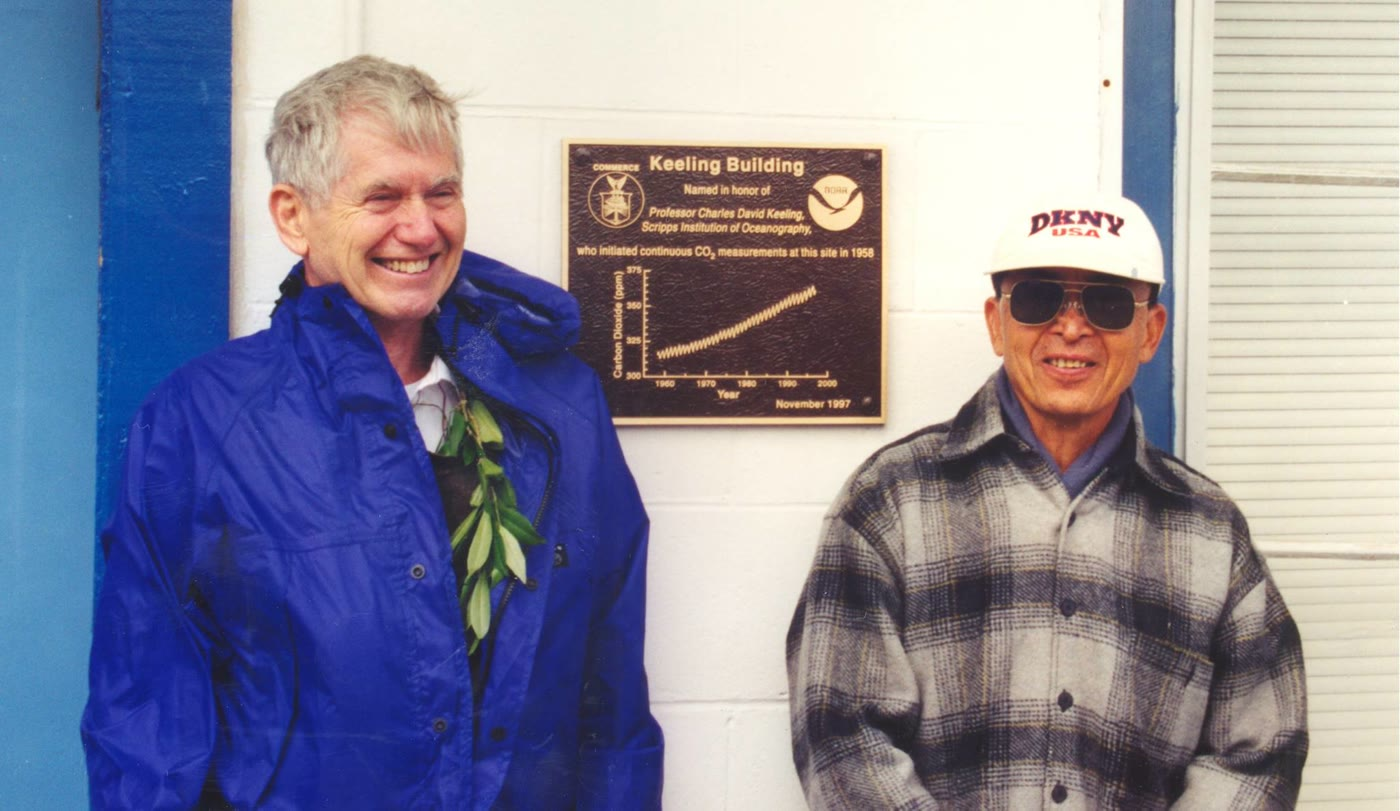
\includegraphics[width=0.62\linewidth]{images/book2/g12-noaa-keeling-chin-1997.jpg}

{\small Charles David Keeling (à esquerda) e John Chin no Observatório de
Mauna Loa em 1997, ao lado da placa que dá o nome de Keeling a um prédio.
Fotografia: John Miller, NOAA (domínio público).}
\end{center}
\end{history}

\section{Exercícios}

\begin{exercise}[$\star$]\label{exo:g12:climate-change:1}
O que é o \omterm{def:g12:climate-change:forcing}{forçamento radiativo} de uma mudança no sistema climático? Em que
unidade ele é medido, e o que significa o seu sinal?
\end{exercise}

\begin{exercise}[$\star$]\label{exo:g12:climate-change:2}
Em que mês do ano a concentração de gás carbônico em Mauna Loa é máxima, e
em qual é mínima? Explique a oscilação anual.
\end{exercise}

\begin{exercise}[$\star$]\label{exo:g12:climate-change:3}
No vocabulário das avaliações, que probabilidade significa \emph{muito
provável}? E \emph{provável}? O que significa uma faixa escrita
$[0.95 \text{ a } 1.20]$?
\end{exercise}

\begin{exercise}[$\star$]\label{exo:g12:climate-change:4}
Da energia extra que o sistema climático ganhou nas últimas décadas, que
parte foi para o oceano? Por que isso explica que o nível do mar suba mesmo
sem derretimento de gelo?
\end{exercise}

\begin{exercise}[$\star$]\label{exo:g12:climate-change:5}
Dê duas \omterm{def:g12:climate-change:feedback}{retroalimentações} climáticas positivas e a resposta negativa que
limita o aquecimento. Explique cada uma numa frase.
\end{exercise}

\begin{exercise}[$\star\star$]\label{exo:g12:climate-change:6}
A concentração média anual de gás carbônico em Mauna Loa foi de
\qty{315.98}{ppm} em 1959 e de \qty{427.35}{ppm} em 2025. Em quantos ppm, e
em que porcentagem, ela aumentou? Qual foi o crescimento médio por ano ao
longo de todo o período?
\end{exercise}

\begin{exercise}[$\star\star$]\label{exo:g12:climate-change:7}
Use a lei logarítmica do capítulo, com $F_{2\times} =
\qty{3.93}{W/m^2}$ e $C_0 = \qty{278}{ppm}$, para calcular o \omterm{def:g12:climate-change:forcing}{forçamento} do
gás carbônico a \qty{427.35}{ppm}, a média anual de 2025.
\end{exercise}

\begin{exercise}[$\star\star$]\label{exo:g12:climate-change:8}
A \qty{3.7}{mm} por ano, a taxa de 2006--2018, quanto o nível do mar subiria
em 30 anos? Quantas vezes mais rápida é essa taxa que a de 1901--1971,
\qty{1.3}{mm} por ano?
\end{exercise}

\begin{exercise}[$\star\star$]\label{exo:g12:climate-change:9}
Usando $\Delta T = F/\lambda$ com $\lambda = \qty{1.16}{W.m^{-2}.\degreeCelsius^{-1}}$,
calcule o aquecimento de equilíbrio que o \omterm{def:g12:climate-change:forcing}{forçamento} humano total de 2019,
\qty{2.72}{W/m^2}, produziria. O aquecimento observado causado pelo homem é
de apenas cerca de \qty{1.07}{\degreeCelsius}. Dê a principal razão da
diferença.
\end{exercise}

\begin{exercise}[$\star\star$]\label{exo:g12:climate-change:10}
O Sol e os vulcões mudaram a temperatura global entre 1850--1900 e
2010--2019 em $-0.1$ a $+\qty{0.1}{\degreeCelsius}$, enquanto o aquecimento
observado foi de cerca de \qty{1.06}{\degreeCelsius}. O que você pode
concluir? Que outra causa natural também deve ser descartada, e o que a
avaliação diz sobre ela?
\end{exercise}

\begin{exercise}[$\star\star$]\label{exo:g12:climate-change:11}
Usando a tabela das projeções, em que \omterm{def:g12:climate-change:scenario}{cenários} o aquecimento de 2081--2100
muito provavelmente fica abaixo de \qty{2}{\degreeCelsius}? Em qual ele muito
provavelmente passa de \qty{2}{\degreeCelsius}?
\end{exercise}

\begin{exercise}[$\star\star\star$]\label{exo:g12:climate-change:12}
Os aerossóis produziram um \omterm{def:g12:climate-change:forcing}{forçamento} de cerca de $-0.22$ e de
$\qty{-0.84}{W/m^2}$ (pela luz do Sol e pelas nuvens). Se todos os
aerossóis fossem retirados do ar e todo o resto continuasse como em 2019,
qual seria o \omterm{def:g12:climate-change:forcing}{forçamento} humano total? Em quanto aumentaria o aquecimento de
equilíbrio, com $\lambda = \qty{1.16}{W.m^{-2}.\degreeCelsius^{-1}}$?
\end{exercise}

\begin{exercise}[$\star\star\star$]\label{exo:g12:climate-change:13}
Mostre, a partir da lei logarítmica, que ir de \qty{278}{ppm} a
\qty{556}{ppm} e ir de \qty{556}{ppm} a \qty{1112}{ppm} acrescentam o mesmo
\omterm{def:g12:climate-change:forcing}{forçamento}. Qual é o \omterm{def:g12:climate-change:forcing}{forçamento} total a \qty{1112}{ppm}?
\end{exercise}

\begin{exercise}[$\star\star\star$]\label{exo:g12:climate-change:14}
Derive a lei logarítmica em relação a $C$. Quanto \omterm{def:g12:climate-change:forcing}{forçamento} acrescenta um
ppm extra de gás carbônico a \qty{280}{ppm}, e quanto a \qty{420}{ppm}?
Comente.
\end{exercise}

\begin{exercise}[$\star\star\star$]\label{exo:g12:climate-change:15}
Sem nenhuma \omterm{def:g12:climate-change:feedback}{retroalimentação} além da radiação extra para o espaço,
$\lambda_0 = \qty{3.22}{W.m^{-2}.\degreeCelsius^{-1}}$. Calcule o aquecimento
para uma duplicação do gás carbônico ($F_{2\times} = \qty{3.93}{W/m^2}$) com
$\lambda_0$, depois com $\lambda = \qty{1.16}{W.m^{-2}.\degreeCelsius^{-1}}$. Por
que fator as \omterm{def:g12:climate-change:feedback}{retroalimentações} amplificam o aquecimento?
\end{exercise}

\section{Problema: a curva de Keeling em números}

\begin{problem}[{Problema de fim de semana --- da respiração anual da
vegetação ao ano em que uma duplicação seria atingida}]
\label{pb:g12:climate-change:1}
% ledger: data:co2-mlo (annual means 1960 316.91, 1970 325.68, 2015 401.01,
% 2025 427.35; seasonal departures May +3.37, September -3.51, means of
% 2015-2024; all from figdata/grade-12/climate_records.py), noaa:mlo-site,
% ipcc:erf-2xco2, ipcc:ecs, ipcc:feedbacks, ipcc:co2-2myr
Um estudante baixa o registro de Mauna Loa e o trabalha com uma planilha. Em
2015--2024, a concentração mensal fica em média \qty{3.37}{ppm} acima da
tendência suavizada em maio e \qty{3.51}{ppm} abaixo dela em setembro. As
médias anuais são de \qty{316.91}{ppm} em 1960, \qty{325.68}{ppm} em 1970,
\qty{401.01}{ppm} em 2015 e \qty{427.35}{ppm}
em 2025. A concentração de 1750 era de \qty{278}{ppm}. Use a lei logarítmica
com $F_{2\times} = \qty{3.93}{W/m^2}$.

\medskip
\noindent\textbf{Parte I --- A respiração da vegetação.}
\begin{enumerate}
  \item Qual é a amplitude de pico a vale do ciclo anual?
  \item Explique por que a concentração é máxima em maio e mínima em
        setembro.
  \item O ciclo é muito mais fraco no ar do Hemisfério Sul. Sugira por quê.
  \item Por que o observatório foi construído a \qty{3397}{m} de altitude,
        num vulcão no meio do Pacífico?
\end{enumerate}

\medskip
\noindent\textbf{Parte II --- A tendência.}
\begin{enumerate}[resume]
  \item Calcule o crescimento médio, em ppm por ano, em 1960--1970.
  \item Calcule-o em 2015--2025.
  \item Por que fator a taxa de crescimento aumentou?
  \item Em que porcentagem a concentração subiu entre 1750 e 2025?
  \item Os \omterm{def:g12:past-climates:ice-core}{testemunhos de gelo} nunca mostram mais de cerca de
        \qty{300}{ppm} nos últimos 800\,000 anos. Em quantos ppm o valor
        de 2025 ultrapassa isso?
\end{enumerate}

\medskip
\noindent\textbf{Parte III --- O forçamento.}
\begin{enumerate}[resume]
  \item Calcule o \omterm{def:g12:climate-change:forcing}{forçamento} do gás carbônico em 2025.
  \item Calcule-o em 1960, e o aumento do \omterm{def:g12:climate-change:forcing}{forçamento} entre 1960 e 2025.
  \item Que concentração acrescentaria \qty{1}{W/m^2} ao \omterm{def:g12:climate-change:forcing}{forçamento} de
        2025?
  \item Na taxa de crescimento de 2015--2025, quantos anos isso levaria?
\end{enumerate}

\medskip
\noindent\textbf{Parte IV --- A duplicação.}
\begin{enumerate}[resume]
  \item Qual é a concentração de uma duplicação do valor de 1750? Que
        \omterm{def:g12:climate-change:forcing}{forçamento} ela produz?
  \item Com a melhor estimativa da \omterm{def:g12:climate-change:ecs}{sensibilidade climática de equilíbrio},
        que aquecimento de equilíbrio ela causaria? Dê a faixa provável.
  \item Que parâmetro de \omterm{def:g12:climate-change:feedback}{retroalimentação} $\lambda$ uma sensibilidade de
        \qty{3}{\degreeCelsius} implica? Compare-o com o valor
        \qty{1.16}{W.m^{-2}.\degreeCelsius^{-1}} obtido somando as
        \omterm{def:g12:climate-change:feedback}{retroalimentações}.
  \item Por que a superfície não atingiria esse aquecimento no dia em que a
        duplicação fosse atingida?
  \item Por que um cálculo que simplesmente prolonga a taxa de crescimento
        de hoje é um \omterm{def:g12:climate-change:scenario}{cenário}, e não uma \omterm{def:g12:climate-change:scenario}{projeção} do tipo que as avaliações
        fazem?
  \item Se a taxa de crescimento de 2015--2025 continuasse a mesma, em que
        ano a duplicação da concentração de 1750 seria atingida?
\end{enumerate}
\end{problem}
